% vim:encoding=utf8 ft=tex sts=2 sw=2 et:

\documentclass{classrep}
\usepackage[utf8]{inputenc}
\usepackage{color}
\usepackage{mathtools}

\usepackage{subfig}
\usepackage{float}

\studycycle{Informatyka, studia niestacjonarne, mgr II st.}
\coursesemester{I}

\coursename{Przetwarzanie obrazu i dźwięku}
\courseyear{2015/2016}

\courseteacher{mgr inż. Piotr Ożdżyński}
\coursegroup{Sobota, 14:15}

\author{
  \studentinfo{Jakub Antosik}{XXXXXX} \and
  \studentinfo{Andrzej Lisowski}{206087} 
}

\title{Zadanie 1: Szkielet aplikacji do przetwarzania i analizy obrazów, operacje podstawowe, usuwanie szumu,
modyfikacje histogramu, filtracja liniowa i nieliniowa, splot.}

\begin{document}
\maketitle

\section{Cel}
Celem zadania było zapoznanie się z metodami analizy i przetwarzania obrazów. W części implementacyjnej należało stworzyć program w wybranym przez siebie języku programowania, który będzie w stanie przeprowadzić różne operacje na obrazie. Pełen spis funkcjonalności zostanie przedstawiony w sekcji \textit{Wprowadzenie}.

\section{Wprowadzenie}
Obraz w pamięci komputera jest reprezentowany przez macierz pikseli. Sam piksel jest zaś najmniejszym elementem obrazu, mogącym przyjmować różne wartości liczb naturalnych:\\
\begin{itemize}
\item 0 - 7 dla obrazów 1-bitowych\\
\item 0 - 255 dla obrazów 8-bitowych (odcienie szarości)\\
\item 0 - 16777215 dla obrazów 24-bitowych (po 8 bitów na każdy kolor RGB)\\
\end{itemize}
Poniżej przedstawione zostały teoretyczne podstawy trasformacji, którym poddane zostały testowe dane.

\subsection{Podstawowe operacje przetwarzania obrazu}
Sekcja ta opisuje podstawowe operacje przetwarzania obrazów, często wykorzystywane w codziennym życiu.

\subsubsection{Zmiana jasności}
Zmiana jasności obrazu polega na dodaniu do wartości każdego piksela pewnej stałej liczby k. Jeżeli stała jest dodatnia, mówimy o zwiększaniu jasności, jeżeli jest ujemna - jasność jest zmniejszana. W momencie, w którym wynik przekroczy wartości brzegowe piksela, przypisuje się mu p$_{\text{min}}$ lub p$_{\text{max}}$ zgodnie z poniższym wzorem:
\[ p(i) =
  \begin{cases}
    p_{min} & \quad \text{jeżeli } i + k < 0\\
    i + k  & \quad \text{jeżeli } p_{min} \leq i+k \leq p_{max}\\
    p_{max}  & \quad \text{jeżeli } i + k > 0\\
  \end{cases}
\]
gdzie:\\
\textit{p(i)} - wartość piksela po zmianie jasności,\\
\textit{i} - wartość piksela przed zmianą jasności,\\
\textit{p$_{\text{min}}$} - minimalna wartość piksela, p$_{\text{min}}$ = 0,\\
\textit{p$_{\text{max}}$} - maksymalna wartość piksela,\\
\textit{k} - zmiana jasności.\\

\subsubsection{Zmiana kontrastu}
Zmiana kontrastu obrazu polega na zwiększeniu jasności jasnych pikseli przy jednoczesnym zmniejszeniu jasności ciemnych pikseli. Ciemne piksele należą do przedziału $\langle$0,$ \frac{p_{max}}{2}$), zaś jasne do przedziału $\langle$$ \frac{p_{max}}{2}$,$p_{max}$$\rangle$.\\
\\
Wzór wygląda następująco:
\[ p(i) =
  \begin{cases}
    i \div k  & \quad \text{jeżeli } 0 \leq i < \frac{p_{max}}{2}\\
    i \ast k  & \quad \text{jeżeli } \frac{p_{max}}{2} \leq i \leq p_{max}\\
    p_{max}  & \quad \text{jeżeli } i \ast k > p_{max}\\
  \end{cases}
\]
gdzie:\\
\textit{p(i)} - wartość piksela po zmianie kontrastu,\\
\textit{i} - wartość piksela przed zmianą kontrastu,\\
\textit{p$_{\text{max}}$} - maksymalna wartość piksela,\\
\textit{k} - współczynnik zmiany kontrastu.\\

\subsubsection{Wyznaczenie negatywu}
Negatyw jest przedstawieniem pikseli obrazu jako różnicy wartości maksymalnej i obecnej:\\
\\
\[p(i) = p_{max} - i\]
gdzie:\\
\textit{p(i)} - wartość piksela po wyznaczeniu negatywu,\\
\textit{i} - wartość piksela przed zmianą kontrastu,\\
\textit{p$_{\text{max}}$} - maksymalna wartość piksela.\\

\subsection{Podstawowe filtry}
Poniższa sekcja opisuje 2 podstawowe filtry, które podległy analizie - filtr ze średnią arytmetyczną oraz filtr medianowy.

\subsubsection{Filtr ze średnią arytmetyczną}
Filtr ze średnią arytmetyczną jest wykorzystywany w operacjach odszumiania obrazu. Algorytm polega na przypisaniu do nowej wartości pikseli średniej arytmetycznej badanego elementu oraz jego sąsiedztwa s. Sąsiedztwo może przyjmować wartości potęg kolejnych liczb nieparzystych większych od 1:\\
\[ s \in \{9,25,49,...\} \]
\[ p(i) = \frac{\displaystyle\sum_{x=-n}^{n}\displaystyle\sum_{y=-n}^{n} i_{x,y}}{s} \]
gdzie:\\
\textit{p(i)} - wartość piksela po nałożeniu filtru,\\
\textit{i} - wartość piksela przed nałożeniem filtru,\\
\textit{s} - maska filtru,\\
\textit{n} - rozpiętość maski filtru, obliczana ze wzoru:\\
\[ n = \frac{\sqrt{s}-1}{2} \]
\textit{x} - współrzędna x piksela na obrazie,\\
\textit{y} - współrzędna y piksela na obrazie.\\
\\
Należy pamiętać, że piksele poddawane filtracji nie mogą być elementami brzegowymi obrazu, więc:
\[ i_x + n \leq x_{max} \wedge i_x - n \geq x_{min} \wedge i_y + n \leq y_{max} \wedge i_y - n \geq y_{min} \]
gdzie:\\
\textit{i} - wartość piksela przed zmianą kontrastu,\\
\textit{x} - współrzędna x piksela na obrazie,\\
\textit{y} - współrzędna y piksela na obrazie,\\
\textit{x$_{\text{max}}$} - maksymalna wartość współrzędnej x na obrazie,\\
\textit{x$_{\text{min}}$} - minimalna wartość współrzędnej x na obrazie, x$_{\text{min}}$ = 0,\\
\textit{y$_{\text{max}}$} - maksymalna wartość współrzędnej y na obrazie,\\
\textit{y$_{\text{min}}$} - minimalna wartość współrzędnej y na obrazie, y$_{\text{min}}$ = 0.\\

\subsubsection{Filtr medianowy}
Filtr medianowy jest bardzo podobny do filtru ze średnią arytmetyczną. W tym przypadku jednak, nowa wartość piksela jest medianą badanego elementu praz jego sąsiedztwa s. Sąsiedztwo może przyjmować wartości potęg kolejnych liczb nieparzystych większych od 1:\\
\[ s \in \{9,25,49,...\} \]
\[ p(i) = M_{s} \]
gdzie:\\
\textit{p(i)} - wartość piksela po nałożeniu filtru,\\
\textit{M} - mediana,\\
\textit{s} - maska filtru.\\
\\
Należy pamiętać, że piksele poddawane filtracji nie mogą być elementami brzegowymi obrazu, więc:
\[ i_x + n \leq x_{max} \wedge i_x - n \geq x_{min} \wedge i_y + n \leq y_{max} \wedge i_y - n \geq y_{min} \]
gdzie:\\
\textit{i} - wartość piksela przed zmianą kontrastu,\\
\textit{n} - rozpiętość maski filtru, obliczana ze wzoru:\\
\[ n = \frac{\sqrt{s}-1}{2} \]
\textit{x} - współrzędna x piksela na obrazie,\\
\textit{y} - współrzędna y piksela na obrazie,\\
\textit{x$_{\text{max}}$} - maksymalna wartość współrzędnej x na obrazie,\\
\textit{x$_{\text{min}}$} - minimalna wartość współrzędnej x na obrazie, x$_{\text{min}}$ = 0,\\
\textit{y$_{\text{max}}$} - maksymalna wartość współrzędnej y na obrazie,\\
\textit{y$_{\text{min}}$} - minimalna wartość współrzędnej y na obrazie, y$_{\text{min}}$ = 0.\\

\subsection{Modyfikacje obrazu w oparciu o histogram}
Histogram umożliwia przedstawienie rozkładu pikseli o określonych wartościach na wykresie. Poniższa sekcja prezentuje modyfikacje obrazu na podstawie jego histogramu.

\subsubsection{Jednostajna wyjściowa gęstość prawdopodobieństwa}
Obliczana jest ze wzoru:
\[ g(f) = g_{min} + (g_{max} - g_{min}) \frac{1}{N} \displaystyle\sum_{m=0}^{f} H(m) \]
gdzie:\\
\textit{f} - wartość rozważanego kanału przed modyfikacją,\\
\textit{g} - wartość rozważanego kanału po modyfikacji,\\
\textit{g$_{\text{min}}$} - pożądana minimalna wartość przetwarzanego kanału,\\
\textit{g$_{\text{max}}$} - pożądana maksymalna wartość przetwarzanego kanału,\\
\textit{N} - suma pikseli na obrazie,\\
\textit{H(m)} - wartość histogramu dla wartości m kanału.\\

\subsubsection{Wyjściowa gęstość prawdopodobieństwa o postaci wykładniczej}
Obliczana jest ze wzoru:
\[ g(f) = g_{min} - \frac{1}{\alpha} ln (1 - \frac{1}{N} \displaystyle\sum_{m=0}^{f} H(m) \]
gdzie:\\
\textit{f} - wartość rozważanego kanału przed modyfikacją,\\
\textit{g} - wartość rozważanego kanału po modyfikacji,\\
\textit{g$_{\text{min}}$} - pożądana minimalna wartość przetwarzanego kanału,\\
\textit{$\alpha$} - współczynnik obiczany ze wzoru: TODO,\\
\textit{N} - suma pikseli na obrazie,\\
\textit{H(m)} - wartość histogramu dla wartości m kanału.\\

\subsubsection{Wyjściowa gęstość prawdopodobieństwa podana wzorem Raleigha}
Obliczana jest ze wzoru:
\[ g(f) = g_{min} + (2 \alpha^2 ln (\frac{1}{N} \displaystyle\sum_{m=0}^{f} H(m))^{-1})^\frac{1}{2} \]
gdzie:\\
\textit{f} - wartość rozważanego kanału przed modyfikacją,\\
\textit{g} - wartość rozważanego kanału po modyfikacji,\\
\textit{g$_{\text{min}}$} - pożądana minimalna wartość przetwarzanego kanału,\\
\textit{$\alpha$} - współczynnik obiczany ze wzoru: TODO,\\
\textit{N} - suma pikseli na obrazie,\\
\textit{H(m)} - wartość histogramu dla wartości m kanału.\\

\subsubsection{Wyjściowa gęstość prawdopodobieństwa określona przez potęgę 2/3}
Obliczana jest ze wzoru:
\[ g(f) = (g_{min}^\frac{1}{3} + (g_{max}^\frac{1}{3} - g_{min}^\frac{1}{3}) \frac{1}{N} \displaystyle\sum_{m=0}^{f} H(m))^3 \]
gdzie:\\
\textit{f} - wartość rozważanego kanału przed modyfikacją,\\
\textit{g} - wartość rozważanego kanału po modyfikacji,\\
\textit{g$_{\text{min}}$} - pożądana minimalna wartość przetwarzanego kanału,\\
\textit{g$_{\text{max}}$} - pożądana maksymalna wartość przetwarzanego kanału,\\
\textit{N} - suma pikseli na obrazie,\\
\textit{H(m)} - wartość histogramu dla wartości m kanału.\\

\subsubsection{Wyjściowa gęstość prawdopodobienstwa o postaci hiperbolicznej}
Obliczana jest ze wzoru:
\[ g(f) = g_{min}(\frac{g_{max}}{g_{min}})^{\frac{1}{N} \displaystyle\sum_{m=0}^{f} H(m)} \]
gdzie:\\
\textit{f} - wartość rozważanego kanału przed modyfikacją,\\
\textit{g} - wartość rozważanego kanału po modyfikacji,\\
\textit{g$_{\text{min}}$} - pożądana minimalna wartość przetwarzanego kanału,\\
\textit{g$_{\text{max}}$} - pożądana maksymalna wartość przetwarzanego kanału,\\
\textit{N} - suma pikseli na obrazie,\\
\textit{H(m)} - wartość histogramu dla wartości m kanału.\\

\subsection{Filtracja liniowa oparta o splot}
Poniższa sekcja przedstawia zbadane przekształcenia filtracji liniowej. Polega ona na modyfikacji pikseli obrazu poprzez nałożenie na nie maski filtrującej. Wzór przedstawia się następująco: 
\[ g(p,q) = \displaystyle\sum_{i=-M}^{M}\displaystyle\sum_{j=-M}^{M} h(i,j)x(p+i,q+j), p = M,2,...,P-M-1, q = M,2,...,Q-M-1 \]
gdzie:\\
\textit{x(p,q)} - wartość rozważanego kanału przed modyfikacją,\\
\textit{g(p,q)} - wartość rozważanego kanału po modyfikacji,\\
\textit{h(i,j)} - wartość maski filtru.\\

\subsubsection{Filtr dolnoprzepustowy}
Filtry dolnoprzepustowe są wykorzystywane do usuwania elementów o wysokiej częstotliwości. Dążą one to uśrednienia wartości sąsiadujących pikselów.
Wykorzystane maski:
\[
\frac{1}{9}
 \begin{pmatrix}
  1 & 1 & 1 \\
  1 & 1 & 1 \\
  1 & 1 & 1 \\
 \end{pmatrix}
\quad
\frac{1}{10}
 \begin{pmatrix}
  1 & 1 & 1 \\
  1 & 2 & 1 \\
  1 & 1 & 1 \\
 \end{pmatrix}
\quad
\frac{1}{16}
 \begin{pmatrix}
  1 & 2 & 1 \\
  2 & 4 & 2 \\
  1 & 2 & 1 \\
 \end{pmatrix}
\]

\subsubsection{Wyostrzanie krawędzi}
Poniższe maski zostały użyte do wyostrzenia krawędzi:
\[
 \begin{pmatrix}
  0 & -1 & 0 \\
  -1 & 5 & -1 \\
  0 & -1 & 0 \\
 \end{pmatrix}
\quad
 \begin{pmatrix}
  -1 & -1 & -1 \\
  -1 & 9 & -1 \\
  -1 & -1 & -1 \\
 \end{pmatrix}
\quad
 \begin{pmatrix}
  1 & -2 & 1 \\
  -2 & 5 & -2 \\
  1 & -2 & 1 \\
 \end{pmatrix}
\]

\subsubsection{Wydobywanie szczegółów z tła: N, NE, E, SE}
Wydobycie szczegółów z tła w kierunkach: północnym, północno-wschodnim, wschodnim i południowo-wschodnim zostało przebadane następującymi maskami:
\[
 \begin{pmatrix}
  1 & 1 & 1 \\
  1 & -2 & 1 \\
  -1 & -1 & -1 \\
 \end{pmatrix}
\quad
 \begin{pmatrix}
  1 & 1 & 1 \\
  -1 & -2 & 1 \\
  -1 & -1 & 1 \\
 \end{pmatrix}
\quad
 \begin{pmatrix}
  -1 & 1 & 1 \\
  -1 & -2 & 1 \\
  -1 & 1 & 1 \\
 \end{pmatrix}
\quad
 \begin{pmatrix}
  -1 & -1 & 1 \\
  -1 & -2 & 1 \\
  1 & 1 & 1 \\
 \end{pmatrix}
\]

\subsubsection{Wydobywanie szczegółów z tła: S, SW, W, NW}
Do wydobycia szczegółów z tła w kierunkach: południowym, południowo-zachodnim, zachodnim i północno-zachodnim zostało wykorzystane następujące maski:
\[
 \begin{pmatrix}
  -1 & -1 & -1 \\
  1 & -2 & 1 \\
  1 & 1 & 1 \\
 \end{pmatrix}
\quad
 \begin{pmatrix}
  1 & -1 & -1 \\
  1 & -2 & -1 \\
  1 & 1 & 1 \\
 \end{pmatrix}
\quad
 \begin{pmatrix}
  1 & 1 & -1 \\
  1 & -2 & -1 \\
  1 & 1 & -1 \\
 \end{pmatrix}
\quad
 \begin{pmatrix}
  1 & 1 & 1 \\
  1 & -2 & -1 \\
  1 & -1 & -1 \\
 \end{pmatrix}
\]

\subsubsection{Wydobywanie szczegółów z tła bez zdefiniowanego kierunku (laplasjan)}
Wydobycie szczegółów z tła bez zdefiniowanego kierunku jest możliwe przy nałożeniu następujących masek:
\[
 \begin{pmatrix}
  0 & -1 & 0 \\
  -1 & 4 & -1 \\
  0 & -1 & 0 \\
 \end{pmatrix}
\quad
 \begin{pmatrix}
  -1 & -1 & -1 \\
  -1 & 8 & -1 \\
  -1 & -1 & -1 \\
 \end{pmatrix}
\quad
 \begin{pmatrix}
  1 & -2 & 1 \\
  -2 & 4 & -2 \\
  1 & -2 & 1 \\
 \end{pmatrix}
\]

\subsubsection{Identyfikowanie linii}
Identyfikowanie linii na obrazie zostało zrealizowane po nałożeniu masek:
\[
 \begin{pmatrix}
  -1 & 2 & -1 \\
  -1 & 2 & -1 \\
  -1 & 2 & -1 \\
 \end{pmatrix}
\quad
 \begin{pmatrix}
  -1 & -1 & -1 \\
  2 & 2 & 2 \\
 -1 & -1 & -1 \\
 \end{pmatrix}
\quad
 \begin{pmatrix}
  -1 & -1 & 2 \\
  -1 & 2 & -1 \\
  2 & -1 & -1 \\
 \end{pmatrix}
\quad
 \begin{pmatrix}
  2 & -1 & -1 \\
  -1 & 2 & -1 \\
  -1 & -1 & 2 \\
 \end{pmatrix}
\]

\subsection{Filtracja nieliniowa}
//TODO

\subsubsection{Operator Robertsa (Wariant I)}
//TODO

\subsubsection{Operator Robertsa (Wariant II)}
//TODO

\subsubsection{Operator Sobela}
//TODO

\subsubsection{Operator Kirsha}
//TODO

\subsubsection{Operator Rosenfelda}
//TODO

\subsubsection{Operator Uolisa}
//TODO

\section{Opis implementacji}
Aplikacja została napisana w języku programowania Java. Wybór środowiska był podyktowany dużą ilością bibliotek mogących pomóc w realizacji zadania oraz osobistymi preferencjami członków zespołu. Warstwa GUI została realizowana przy użyciu standardowej bilbioteki graficznej Javy - Swing. Aplikacja wykorzystuje następujące bilbioteki zewnętrzne:
\begin{itemize}
\item \textit{JavaPlot.jar} - wykorzystywana do tworzenia histogramów; jest to javowa implementacja gnuplota 
\item \textit{log4j-1.2.17.jar} - wykorzystywana do obsługi logowania
\item \textit{slf4j-api-1.7.12.jar} - wykorzystywana do obsługi logowania
\item \textit{slf4j-log4j12-1.7.12.jar} - wykorzystywana do obsługi logowania
\end{itemize}

Poniżej przedstawiony został diagram UML klas znajdujących się w programie. Aby zachować czytelność, nie zamieszczono połączeń pomiędzy wywołaniami obiektów, a także ukryto informacje na temat metod i parametrów.

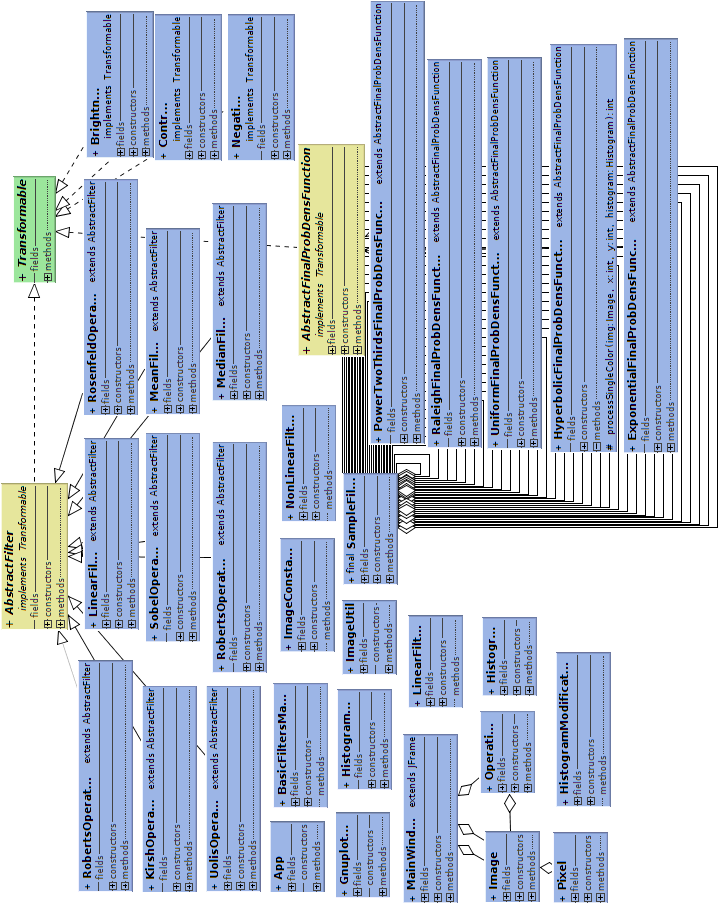
\includegraphics[scale=0.6]{img/uml_diagram.png}

\section{Materiały i metody}
Testowy zbiór przekształcanych obrazów można podzielić na 3 główne grupy:
\begin{itemize}
\item obrazy 1-bitowe
\begin{figure}%
    \centering
    \subfloat[Boat]{{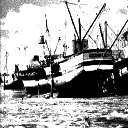
\includegraphics[width=2.5cm,height=2.5cm,keepaspectratio]{img/original/bit1/boatbw_small.png}}}%
    \qquad
    \subfloat[Girl]{{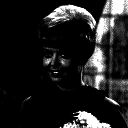
\includegraphics[width=2.5cm,height=2.5cm,keepaspectratio]{img/original/bit1/girlbw_small.png}}}%
    \qquad
    \subfloat[Lena]{{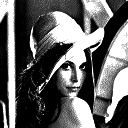
\includegraphics[width=2.5cm,height=2.5cm,keepaspectratio]{img/original/bit1/lenabw_small.png}}}%
    \qquad
    \subfloat[Mandril]{{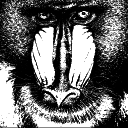
\includegraphics[width=2.5cm,height=2.5cm,keepaspectratio]{img/original/bit1/mandrilbw_small.png}}}%
    \caption{Testowe obrazy 1-bitowe}%
\end{figure}
\item obrazy 8-bitowe (w skali szarości)
\begin{figure}%
    \centering
    \subfloat[Aero]{{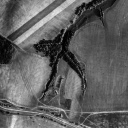
\includegraphics[width=2.5cm,height=2.5cm,keepaspectratio]{img/original/bit8/aero_small.png}}}%
    \qquad
    \subfloat[Bird]{{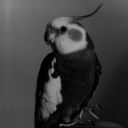
\includegraphics[width=2.5cm,height=2.5cm,keepaspectratio]{img/original/bit8/bird_small.png}}}%
    \qquad
    \subfloat[Boat]{{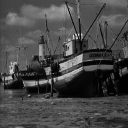
\includegraphics[width=2.5cm,height=2.5cm,keepaspectratio]{img/original/bit8/boat_small.png}}}%
    \qquad
    \subfloat[Bridge]{{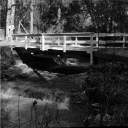
\includegraphics[width=2.5cm,height=2.5cm,keepaspectratio]{img/original/bit8/bridge_small.png}}}%
    \qquad
    \subfloat[Camera]{{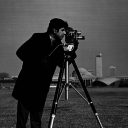
\includegraphics[width=2.5cm,height=2.5cm,keepaspectratio]{img/original/bit8/camera_small.png}}}%
    \qquad
    \subfloat[Lena]{{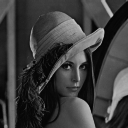
\includegraphics[width=2.5cm,height=2.5cm,keepaspectratio]{img/original/bit8/lena_small.png}}}%
    \qquad
    \subfloat[Mandril]{{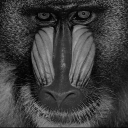
\includegraphics[width=2.5cm,height=2.5cm,keepaspectratio]{img/original/bit8/mandril_small.png}}}%
    \qquad
    \subfloat[Messer]{{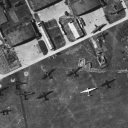
\includegraphics[width=2.5cm,height=2.5cm,keepaspectratio]{img/original/bit8/messer_small.png}}}%
    \qquad
    \subfloat[Pentagon]{{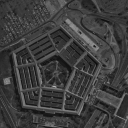
\includegraphics[width=2.5cm,height=2.5cm,keepaspectratio]{img/original/bit8/pentagon_small.png}}}%
    \caption{Testowe obrazy 8-bitowe}%
\end{figure}
\begin{figure}%
    \centering
    \subfloat[Impulsowy 1]{{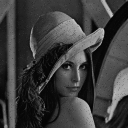
\includegraphics[width=2.5cm,height=2.5cm,keepaspectratio]{img/original/bit8/noise/lena_impulse1_small.png}}}%
    \qquad
    \subfloat[Impulsowy 2]{{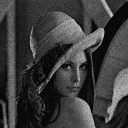
\includegraphics[width=2.5cm,height=2.5cm,keepaspectratio]{img/original/bit8/noise/lena_impulse2_small.png}}}%
    \qquad
    \subfloat[Impulsowy 3]{{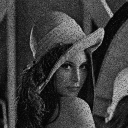
\includegraphics[width=2.5cm,height=2.5cm,keepaspectratio]{img/original/bit8/noise/lena_impulse3_small.png}}}%
    \qquad
    \subfloat[Normalny 1]{{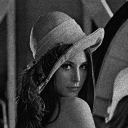
\includegraphics[width=2.5cm,height=2.5cm,keepaspectratio]{img/original/bit8/noise/lena_normal1_small.png}}}%
    \qquad
    \subfloat[Normalny 2]{{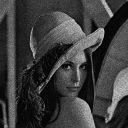
\includegraphics[width=2.5cm,height=2.5cm,keepaspectratio]{img/original/bit8/noise/lena_normal2_small.png}}}%
    \qquad
    \subfloat[Normalny 3]{{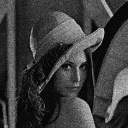
\includegraphics[width=2.5cm,height=2.5cm,keepaspectratio]{img/original/bit8/noise/lena_normal3_small.png}}}%
    \qquad
    \subfloat[Jednolity 1]{{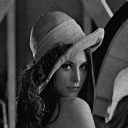
\includegraphics[width=2.5cm,height=2.5cm,keepaspectratio]{img/original/bit8/noise/lena_uniform1_small.png}}}%
    \qquad
    \subfloat[Jednolity 2]{{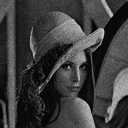
\includegraphics[width=2.5cm,height=2.5cm,keepaspectratio]{img/original/bit8/noise/lena_uniform2_small.png}}}%
    \qquad
    \subfloat[Jednolity 3]{{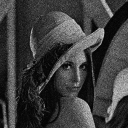
\includegraphics[width=2.5cm,height=2.5cm,keepaspectratio]{img/original/bit8/noise/lena_uniform3_small.png}}}%
    \caption{Testowe obrazy Lena 8-bitowe zaszumione}%
\end{figure}
\item obrazy 24-bitowe (RGB)
\begin{figure}%
    \centering
    \subfloat[Girl]{{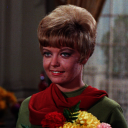
\includegraphics[width=2.5cm,height=2.5cm,keepaspectratio]{img/original/bit24/girlc_small.png}}}%
    \qquad
    \subfloat[Lena]{{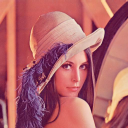
\includegraphics[width=2.5cm,height=2.5cm,keepaspectratio]{img/original/bit24/lenac_small.png}}}%
    \qquad
    \subfloat[Mandril]{{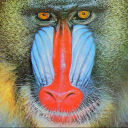
\includegraphics[width=2.5cm,height=2.5cm,keepaspectratio]{img/original/bit24/mandrilc_small.png}}}%
    \caption{Testowe obrazy 24-bitowe}%
\end{figure}
\begin{figure}%
    \centering
    \subfloat[Impulsowy 1]{{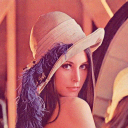
\includegraphics[width=2.5cm,height=2.5cm,keepaspectratio]{img/original/bit24/noise/lenac_impulse1_small.png}}}%
    \qquad
    \subfloat[Impulsowy 2]{{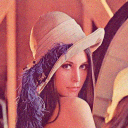
\includegraphics[width=2.5cm,height=2.5cm,keepaspectratio]{img/original/bit24/noise/lenac_impulse2_small.png}}}%
    \qquad
    \subfloat[Impulsowy 3]{{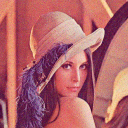
\includegraphics[width=2.5cm,height=2.5cm,keepaspectratio]{img/original/bit24/noise/lenac_impulse3_small.png}}}%
    \qquad
    \subfloat[Normalny 1]{{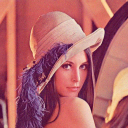
\includegraphics[width=2.5cm,height=2.5cm,keepaspectratio]{img/original/bit24/noise/lenac_normal1_small.png}}}%
    \qquad
    \subfloat[Normalny 2]{{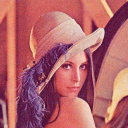
\includegraphics[width=2.5cm,height=2.5cm,keepaspectratio]{img/original/bit24/noise/lenac_normal2_small.png}}}%
    \qquad
    \subfloat[Normalny 3]{{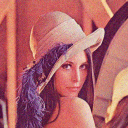
\includegraphics[width=2.5cm,height=2.5cm,keepaspectratio]{img/original/bit24/noise/lenac_normal3_small.png}}}%
    \qquad
    \subfloat[Jednolity 1]{{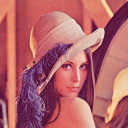
\includegraphics[width=2.5cm,height=2.5cm,keepaspectratio]{img/original/bit24/noise/lenac_uniform1_small.png}}}%
    \qquad
    \subfloat[Jednolity 2]{{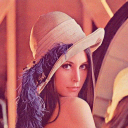
\includegraphics[width=2.5cm,height=2.5cm,keepaspectratio]{img/original/bit24/noise/lenac_uniform2_small.png}}}%
    \qquad
    \subfloat[Jednolity 3]{{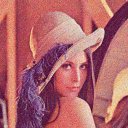
\includegraphics[width=2.5cm,height=2.5cm,keepaspectratio]{img/original/bit24/noise/lenac_uniform3_small.png}}}%
    \caption{Testowe obrazy Lena 24-bitowe zaszumione}%
\end{figure}
\end{itemize}

Badania zostały zrealizowane przy pomocy stworzonej aplikacji. Użytkownik definiował wejściowy obraz, który potem był poddawany wybranemu przez niego przekształceniu. Wyniki były zapisywane na dysku. Szczegółowa konfiguracja współczynników podczas transformacji zostanie podany w sekcji \textit{Wyniki}.

\section{Wyniki}
Poniżej przedstawione zostały efekty przeprowadzonych badań. Przeanalizowano wybrane obrazy 1-, 8- i 24-bitowe.

\subsection{Podstawowe operacje przetwarzania obrazu}
Sekcja przedstawia wyniki podstawowego przetwarzania obrazów - zmiany jasności, kontrastu oraz wyznaczenia negatywu.

\subsubsection{Zmiana jasności}
Poniżej przedstawione zostały wyniki zmiany jasności dla 3 wybranych obrazów.
\begin{figure}[H]%
    \centering
    \subfloat[k = -100]{{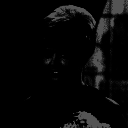
\includegraphics[width=2.5cm,height=2.5cm,keepaspectratio]{img/transformed/basic/brightness/brightness_girl_1_100_minus.png}}}%
    \qquad
    \subfloat[k = -50]{{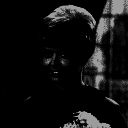
\includegraphics[width=2.5cm,height=2.5cm,keepaspectratio]{img/transformed/basic/brightness/brightness_girl_1_50_minus.png}}}%
      \qquad
    \subfloat[k = 50]{{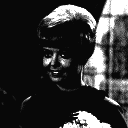
\includegraphics[width=2.5cm,height=2.5cm,keepaspectratio]{img/transformed/basic/brightness/brightness_girl_1_50_plus.png}}}%
    \qquad
    \subfloat[k = 100]{{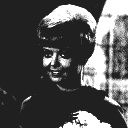
\includegraphics[width=2.5cm,height=2.5cm,keepaspectratio]{img/transformed/basic/brightness/brightness_girl_1_100_plus.png}}}%
    \caption{Zmiana jasności w obrazie Girl 1-bitowym}%
\end{figure}

\begin{figure}[H]%
    \centering
    \subfloat[k = -100]{{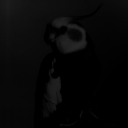
\includegraphics[width=2.5cm,height=2.5cm,keepaspectratio]{img/transformed/basic/brightness/brightness_bird_8_100_minus.png}}}%
    \qquad
    \subfloat[k = -50]{{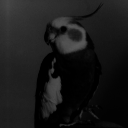
\includegraphics[width=2.5cm,height=2.5cm,keepaspectratio]{img/transformed/basic/brightness/brightness_bird_8_50_minus.png}}}%
      \qquad
    \subfloat[k = 50]{{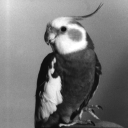
\includegraphics[width=2.5cm,height=2.5cm,keepaspectratio]{img/transformed/basic/brightness/brightness_bird_8_50_plus.png}}}%
    \qquad
    \subfloat[k = 100]{{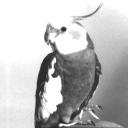
\includegraphics[width=2.5cm,height=2.5cm,keepaspectratio]{img/transformed/basic/brightness/brightness_bird_8_100_plus.png}}}%
    \caption{Zmiana jasności w obrazie Bird 8-bitowym}%
\end{figure}
\begin{figure}[H]%
    \centering
    \subfloat[k = -100]{{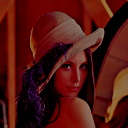
\includegraphics[width=2.5cm,height=2.5cm,keepaspectratio]{img/transformed/basic/brightness/brightness_lena_24_100_minus.png}}}%
    \qquad
    \subfloat[k = -50]{{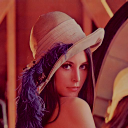
\includegraphics[width=2.5cm,height=2.5cm,keepaspectratio]{img/transformed/basic/brightness/brightness_lena_24_50_minus.png}}}%
      \qquad
    \subfloat[k = 50]{{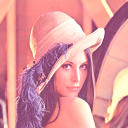
\includegraphics[width=2.5cm,height=2.5cm,keepaspectratio]{img/transformed/basic/brightness/brightness_lena_24_50_plus.png}}}%
    \qquad
    \subfloat[k = 100]{{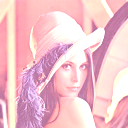
\includegraphics[width=2.5cm,height=2.5cm,keepaspectratio]{img/transformed/basic/brightness/brightness_lena_24_100_plus.png}}}%
    \caption{Zmiana jasności w obrazie Lena 24-bitowym}%
\end{figure}

\subsubsection{Zmiana kontrastu}
Poniżej przedstawione zostały wyniki zmiany kontrastu dla 3 wybranych obrazów.
\begin{figure}[H]%
    \centering
    \subfloat[k = 0.5]{{
\includegraphics[width=2.5cm,height=2.5cm,keepaspectratio]{img/transformed/basic/contrast/contrast_boat_1_0_5.png}}}%
    \qquad
    \subfloat[k = 0.75]{{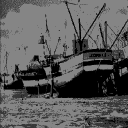
\includegraphics[width=2.5cm,height=2.5cm,keepaspectratio]{img/transformed/basic/contrast/contrast_boat_1_0_75.png}}}%
     \qquad
    \subfloat[k = 1.25]{{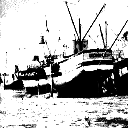
\includegraphics[width=2.5cm,height=2.5cm,keepaspectratio]{img/transformed/basic/contrast/contrast_boat_1_1_25.png}}}%
    \qquad
    \subfloat[k = 1.5]{{\includegraphics[width=2.5cm,height=2.5cm,keepaspectratio]{img/transformed/basic/contrast/contrast_boat_1_1_5.png}}}%
    \caption{Zmiana kontrastu w obrazie Boat 1-bitowym}%
\end{figure}

\begin{figure}[H]%
    \centering
    \subfloat[k = 0.5]{{\includegraphics[width=2.5cm,height=2.5cm,keepaspectratio]{img/transformed/basic/contrast/contrast_aero_8_0_5.png}}}%
    \qquad
    \subfloat[k = 0.75]{{\includegraphics[width=2.5cm,height=2.5cm,keepaspectratio]{img/transformed/basic/contrast/contrast_aero_8_0_75.png}}}%
     \qquad
    \subfloat[k = 1.25]{{\includegraphics[width=2.5cm,height=2.5cm,keepaspectratio]{img/transformed/basic/contrast/contrast_aero_8_1_25.png}}}%
    \qquad
    \subfloat[k = 1.5]{{\includegraphics[width=2.5cm,height=2.5cm,keepaspectratio]{img/transformed/basic/contrast/contrast_aero_8_1_5.png}}}%
    \caption{Zmiana kontrastu w obrazie Aero 8-bitowym}%
\end{figure}

\begin{figure}[H]%
    \centering
    \subfloat[k = 0.5]{{\includegraphics[width=2.5cm,height=2.5cm,keepaspectratio]{img/transformed/basic/contrast/contrast_mandril_24_0_5.png}}}%
    \qquad
    \subfloat[k = 0.75]{{\includegraphics[width=2.5cm,height=2.5cm,keepaspectratio]{img/transformed/basic/contrast/contrast_mandril_24_0_75.png}}}%
     \qquad
    \subfloat[k = 1.25]{{\includegraphics[width=2.5cm,height=2.5cm,keepaspectratio]{img/transformed/basic/contrast/contrast_mandril_24_1_25.png}}}%
    \qquad
    \subfloat[k = 1.5]{{\includegraphics[width=2.5cm,height=2.5cm,keepaspectratio]{img/transformed/basic/contrast/contrast_mandril_24_1_5.png}}}%
    \caption{Zmiana kontrastu w obrazie Mandril 24-bitowym}%
\end{figure}

\subsubsection{Wyznaczenie negatywu}
Poniżej przedstawione zostały wyniki wyznaczenia negatywu dla 3 wybranych obrazów.
\begin{figure}[H]%
    \centering
    \subfloat[Boat 1b]{{\includegraphics[width=2.5cm,height=2.5cm,keepaspectratio]{img/transformed/basic/negative/negative_boat_1.png}}}%
    \qquad
    \subfloat[Camera 8b]{{\includegraphics[width=2.5cm,height=2.5cm,keepaspectratio]{img/transformed/basic/negative/negative_camera_8.png}}}%
    \qquad
    \subfloat[Mandril 24b]{{\includegraphics[width=2.5cm,height=2.5cm,keepaspectratio]{img/transformed/basic/negative/negative_mandril_24.png}}}%
    \caption{Negatyw wybranych obrazów}%
\end{figure}


\subsection{Podstawowe filtry}
//TODO

\subsubsection{Filtr ze średnią arytmetyczną}
//TODO

\subsubsection{Filtr medianowy}
//TODO

\subsection{Modyfikacje obrazu w oparciu o histogram}
//TODO

\subsubsection{Jednostajna wyjściowa gęstość prawdopodobieństwa}
//TODO

\subsubsection{Wyjściowa gęstość prawdopodobieństwa o postaci wykładniczej}
//TODO

\subsubsection{Wyjściowa gęstość prawdopodobieństwa podana wzorem Raleigha}
//TODO

\subsubsection{Wyjściowa gęstość prawdopodobieństwa określona przez potęgę 2/3}
//TODO

\subsubsection{Wyjściowa gęstość prawdopodobienstwa o postaci hiperbolicznej}
//TODO

\subsection{Filtracja liniowa oparta o splot}
//TODO

\subsubsection{Filtr dolnoprzepustowy}
//TODO

\subsubsection{Wyostrzanie krawędzi}
//TODO

\subsubsection{Wydobywanie szczegółów z tła: N, NE, E, SE}
//TODO

\subsubsection{Wydobywanie szczegółów z tła: S, SW, W, NW}
//TODO

\subsubsection{Wydobywanie szczegółów z tła bez zdefiniowanego kierunku (laplasjan)}
//TODO

\subsubsection{Identyfikowanie linii}
//TODO

\subsection{Filtracja nieliniowa}
//TODO

\subsubsection{Operator Robertsa (Wariant I)}
//TODO

\subsubsection{Operator Sobela}
//TODO

\subsubsection{Operator Kirsha}
//TODO

\subsubsection{Operator Rosenfelda}
//TODO

\subsubsection{Operator Uolisa}
//TODO


{\color{blue}
W tej sekcji należy zaprezentować, dla każdego przeprowadzonego eksperymentu,
kompletny zestaw wyników w postaci tabel, wykresów itp. Powinny być one tak
ponazywane, aby było wiadomo, do czego się odnoszą. Wszystkie tabele i wykresy
należy oczywiście opisać (opisać co jest na osiach, w kolumnach itd.) stosując
się do przyjętych wcześniej oznaczeń. Nie należy tu komentować i interpretować
wyników, gdyż miejsce na to jest w kolejnej sekcji. Tu również dobrze jest
wprowadzić oznaczenia (tabel, wykresów) aby móc się do nich odwoływać
poniżej.}

\section{Dyskusja}
{\color{blue}
Sekcja ta powinna zawierać dokładną interpretację uzyskanych wyników
eksperymentów wraz ze szczegółowymi wnioskami z nich płynącymi. Najcenniejsze
są, rzecz jasna, wnioski o charakterze uniwersalnym, które mogą być istotne
przy innych, podobnych zadaniach. Należy również omówić i wyjaśnić wszystkie
napotakane problemy (jeśli takie były). Każdy wniosek powinien mieć poparcie
we wcześniej przeprowadzonych eksperymentach (odwołania do konkretnych
wyników). Jest to jedna z najważniejszych sekcji tego sprawozdania, gdyż
prezentuje poziom zrozumienia badanego problemu.}
\section{Wnioski}
{\color{blue}W tej, przedostatniej, sekcji należy zamieścić podsumowanie
najważniejszych wniosków z sekcji poprzedniej. Najlepiej jest je po prostu
wypunktować. Znów, tak jak poprzednio, najistotniejsze są wnioski o
charakterze uniwersalnym.}


\begin{thebibliography}{1}
\bibitem{instruction_pol}\text{$http://ftims.edu.p.lodz.pl/pluginfile.php/18220/mod\_resource/content/1/$}\\
\text{$Zadanie1.pdf, 2015$}

\bibitem{instruction_ang}\text{$http://ics.p.lodz.pl/~tomczyk/available/po\_en/second.html, 2015$}

\bibitem{instruction_latex}\text{$https://en.wikibooks.org/wiki/LaTeX/Mathematics, 2015$}

\bibitem{doc_linear_fitering}\text{$https://pl.wikipedia.org/wiki/Filtracja\_obraz\%C3\%B3w, 2015$}
\end{thebibliography}
\end{document}
